\documentclass{article}
\usepackage{tikz}
\usetikzlibrary{shapes}

\usetikzlibrary{arrows}
\tikzset{
	treenode/.style = {align=center, inner sep=0pt, text centered,
		font=\sffamily},
	arn_n/.style = {treenode, circle, white, font=\sffamily\bfseries, draw=black,
		fill=black, text width=1.5em},% arbre rouge noir, noeud noir
	arn_r/.style = {treenode, circle, red, draw=red, 
		text width=1.5em, very thick},% arbre rouge noir, noeud rouge
	arn_x/.style = {treenode, rectangle, draw=black,
		minimum width=0.5em, minimum height=0.5em}% arbre rouge noir, nil
}


\usepackage{fancyvrb}  % for the Verbatim environment
\usepackage{graphicx}  % to include graphics
\usepackage{hyperref}  % for hyperlinks

\title{CS200 Functional Data Structures\\Assignment 2}
\author{Beep Beep: Affan-am00634 and Affan-sa00310}


\begin{document}
\maketitle
\section*{Problem 1. Red Black Tree}
	Please see the ass2.hs file in the same folder.
\section*{Problem 2. Insertion}
\begin{enumerate}
	\item 2-4 Tree

	\begin{enumerate}
		\item We begin with an empty tree.
			
\begin{tikzpicture}
			\tikzstyle{bplus}=[rectangle split, rectangle split horizontal,rectangle split ignore empty parts,draw]
			\tikzstyle{every node}=[bplus]
			\tikzstyle{level 1}=[sibling distance=60mm]
			\tikzstyle{level 2}=[sibling distance=15mm]
			
			\node {NULL}
			;\end{tikzpicture}
		\item Insert(1)
			
\begin{tikzpicture}
			\tikzstyle{bplus}=[rectangle split, rectangle split horizontal,rectangle split ignore empty parts,draw]
			\tikzstyle{every node}=[bplus]
			\tikzstyle{level 1}=[sibling distance=60mm]
			\tikzstyle{level 2}=[sibling distance=15mm]
			
			\node {1}
			;\end{tikzpicture}
		\item Insert(24)
			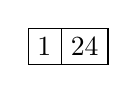
\begin{tikzpicture}
			\tikzstyle{bplus}=[rectangle split, rectangle split horizontal,rectangle split ignore empty parts,draw]
			\tikzstyle{every node}=[bplus]
			\tikzstyle{level 1}=[sibling distance=60mm]
			\tikzstyle{level 2}=[sibling distance=15mm]
			
			\node {1 \nodepart{two} 24}
			;\end{tikzpicture}
		\item Insert(2) \textit{(after rearrangement)}
			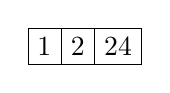
\begin{tikzpicture}
			\tikzstyle{bplus}=[rectangle split, rectangle split horizontal,rectangle split ignore empty parts,draw]
			\tikzstyle{every node}=[bplus]
			\tikzstyle{level 1}=[sibling distance=60mm]
			\tikzstyle{level 2}=[sibling distance=15mm]
			
			\node {1 \nodepart{two} 2 \nodepart{three} 24}
			;\end{tikzpicture}
			
		\item Insert(6)
			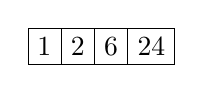
\begin{tikzpicture}
			\tikzstyle{bplus}=[rectangle split, rectangle split horizontal,rectangle split ignore empty parts,draw]
			\tikzstyle{every node}=[bplus]
			\tikzstyle{level 1}=[sibling distance=60mm]
			\tikzstyle{level 2}=[sibling distance=15mm]
			
			\node {1 \nodepart{two} 2 \nodepart{three} 6 \nodepart{four} 24 }
			;\end{tikzpicture}\\
			Break parent;\\
			\begin{tikzpicture}
			\tikzstyle{bplus}=[rectangle split, rectangle split horizontal,rectangle split ignore empty parts,draw]
			\tikzstyle{every node}=[bplus]
			\tikzstyle{level 1}=[sibling distance=60mm]
			\tikzstyle{level 2}=[sibling distance=15mm]
			
			\node {2} [->]
			child {node {1}}
				child {node {6 \nodepart{two} 24}}
			
			;\end{tikzpicture}
		\item Insert(4)\\
			\begin{tikzpicture}
			\tikzstyle{bplus}=[rectangle split, rectangle split horizontal,rectangle split ignore empty parts,draw]
			\tikzstyle{every node}=[bplus]
			\tikzstyle{level 1}=[sibling distance=60mm]
			\tikzstyle{level 2}=[sibling distance=15mm]
			
			\node {2} [->]
			child {node {1}}
			child {node {4 \nodepart{two} 6 \nodepart{three} 24}}
			;\end{tikzpicture}
		\item Insert(12)\\
			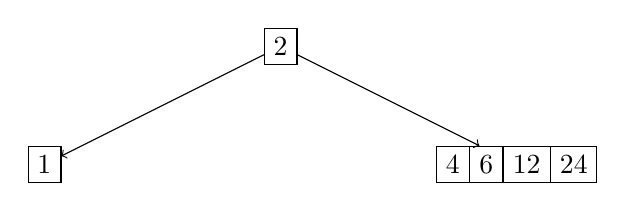
\begin{tikzpicture}
			\tikzstyle{bplus}=[rectangle split, rectangle split horizontal,rectangle split ignore empty parts,draw]
			\tikzstyle{every node}=[bplus]
			\tikzstyle{level 1}=[sibling distance=60mm]
			\tikzstyle{level 2}=[sibling distance=15mm]
			
			\node {2} [->]
			child {node {1}}
			child {node {4 \nodepart{two} 6 \nodepart{three} 12 \nodepart{four} 24}}
			;\end{tikzpicture}
			\\After breaking node 6\\
				\begin{tikzpicture}
				\tikzstyle{bplus}=[rectangle split, rectangle split horizontal,rectangle split ignore empty parts,draw]
				\tikzstyle{every node}=[bplus]
				\tikzstyle{level 1}=[sibling distance=60mm]
				\tikzstyle{level 2}=[sibling distance=15mm]
				
				\node {2} [->]
				child {node {1}}
				child {node {6}
					child{ node{4}}
					child{ node{12 \nodepart {two} 24}}
				}
				
			;\end{tikzpicture}
		\\ Pushing 6 up.\\
					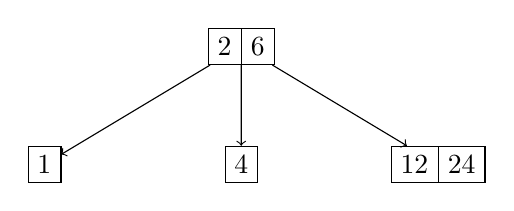
\begin{tikzpicture}
					\tikzstyle{bplus}=[rectangle split, rectangle split horizontal,rectangle split ignore empty parts,draw]
					\tikzstyle{every node}=[bplus]
					\tikzstyle{level 1}=[sibling distance=60mm]
					\tikzstyle{level 2}=[sibling distance=15mm]
					
					\node {2 \nodepart{two} 6} [->]
					child[sibling distance = 25mm] {node {1}}
					child[sibling distance = 25mm] {node {4}}
					child[sibling distance = 25mm]{ node{12 \nodepart {two} 24}}
					
					;\end{tikzpicture}
		\item Insert(25) \textit{trivial}\\
				
				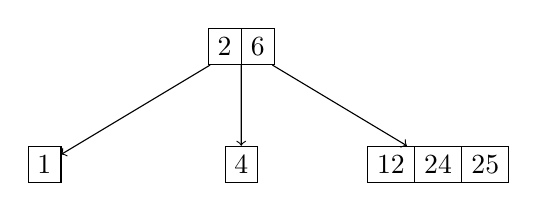
\begin{tikzpicture}
				\tikzstyle{bplus}=[rectangle split, rectangle split horizontal,rectangle split ignore empty parts,draw]
				\tikzstyle{every node}=[bplus]
				\tikzstyle{level 1}=[sibling distance=60mm]
				\tikzstyle{level 2}=[sibling distance=15mm]
				
				\node {2 \nodepart{two} 6} [->]
				child[sibling distance = 25mm] {node {1}}
				child[sibling distance = 25mm] {node {4}}
				child[sibling distance = 25mm]{ node{12 \nodepart {two} 24 \nodepart{three}25}
				}
				
				;\end{tikzpicture}
		\item Insert(19)\\
				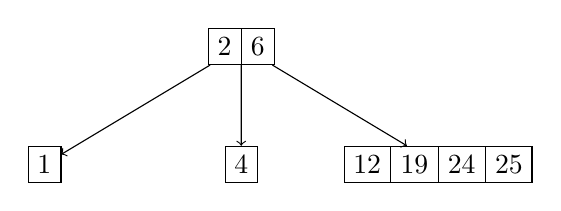
\begin{tikzpicture}
				\tikzstyle{bplus}=[rectangle split, rectangle split horizontal,rectangle split ignore empty parts,draw]
				\tikzstyle{every node}=[bplus]
				\tikzstyle{level 1}=[sibling distance=60mm]
				\tikzstyle{level 2}=[sibling distance=15mm]
				
				\node {2 \nodepart{two} 6} [->]
				child[sibling distance = 25mm] {node {1}}
				child[sibling distance = 25mm] {node {4}}
				child[sibling distance = 25mm]{ node{12 \nodepart{two} 19 \nodepart {three} 24 \nodepart{four}25}}
				
				;\end{tikzpicture}
		\\Breaking 19 and pushing it up\\
			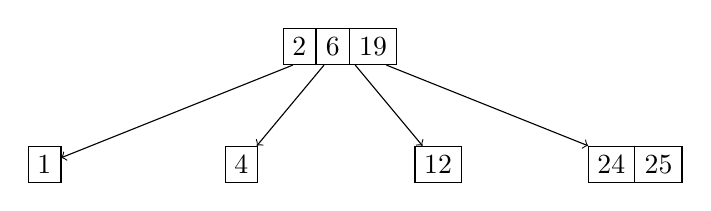
\begin{tikzpicture}
			\tikzstyle{bplus}=[rectangle split, rectangle split horizontal,rectangle split ignore empty parts,draw]
			\tikzstyle{every node}=[bplus]
			\tikzstyle{level 1}=[sibling distance=60mm]
			\tikzstyle{level 2}=[sibling distance=15mm]
			
			\node {2 \nodepart{two} 6 \nodepart{three}19} [->]
			child[sibling distance = 25mm] {node {1}}
			child[sibling distance = 25mm] {node {4}}
			child[sibling distance = 25mm]{ node{12}}
			child[sibling distance = 25mm]{ node{24  \nodepart {two} 25}}
			
			;\end{tikzpicture}
		\item Insert (10) \textit{trivial}\\
			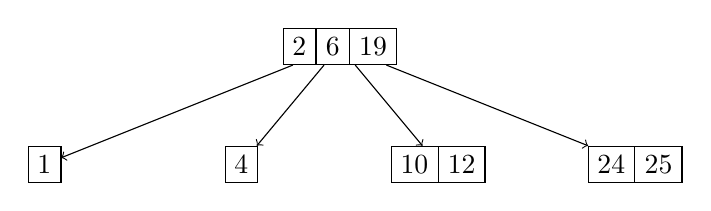
\begin{tikzpicture}
			\tikzstyle{bplus}=[rectangle split, rectangle split horizontal,rectangle split ignore empty parts,draw]
			\tikzstyle{every node}=[bplus]
			\tikzstyle{level 1}=[sibling distance=60mm]
			\tikzstyle{level 2}=[sibling distance=15mm]
			
			\node {2 \nodepart{two} 6 \nodepart{three}19} [->]
			child[sibling distance = 25mm] {node {1}}
			child[sibling distance = 25mm] {node {4}}
			child[sibling distance = 25mm]{ node{ 10 \nodepart{two}12}}
			child[sibling distance = 25mm]{ node{24  \nodepart {two} 25}}
			
			;\end{tikzpicture}
		\item Insert(5) \textit{trivial}\\
			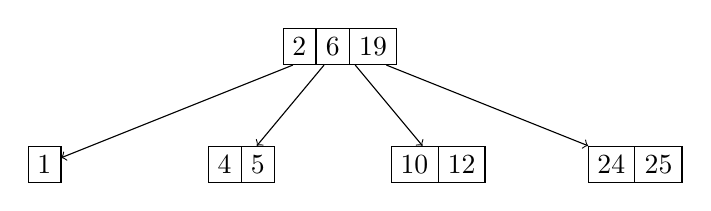
\begin{tikzpicture}
			\tikzstyle{bplus}=[rectangle split, rectangle split horizontal,rectangle split ignore empty parts,draw]
			\tikzstyle{every node}=[bplus]
			\tikzstyle{level 1}=[sibling distance=60mm]
			\tikzstyle{level 2}=[sibling distance=15mm]
			
			\node {2 \nodepart{two} 6 \nodepart{three}19} [->]
			child[sibling distance = 25mm] {node {1}}
			child[sibling distance = 25mm] {node {4 \nodepart{two} 5}}
			child[sibling distance = 25mm]{ node{ 10 \nodepart{two}12}}
			child[sibling distance = 25mm]{ node{24  \nodepart {two} 25}}
			
			;\end{tikzpicture}
		\item Insert(3) \textit{trivial}\\
				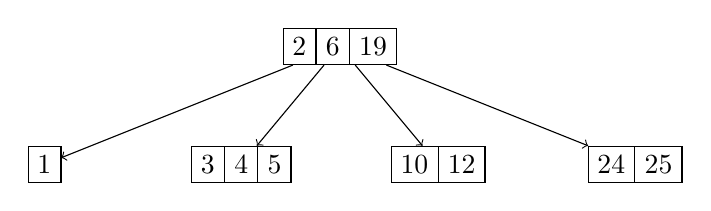
\begin{tikzpicture}
				\tikzstyle{bplus}=[rectangle split, rectangle split horizontal,rectangle split ignore empty parts,draw]
				\tikzstyle{every node}=[bplus]
				\tikzstyle{level 1}=[sibling distance=60mm]
				\tikzstyle{level 2}=[sibling distance=15mm]
				
				\node {2 \nodepart{two} 6 \nodepart{three}19} [->]
				child[sibling distance = 25mm] {node {1}}
				child[sibling distance = 25mm] {node {3 \nodepart{two}4 \nodepart{three} 5}}
				child[sibling distance = 25mm]{ node{ 10 \nodepart{two}12}}
				child[sibling distance = 25mm]{ node{24  \nodepart {two} 25}}
				
				;\end{tikzpicture}
		\item Insert(13) \textit{trivial}\\
					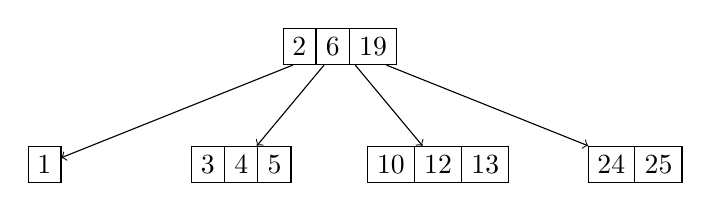
\begin{tikzpicture}
					\tikzstyle{bplus}=[rectangle split, rectangle split horizontal,rectangle split ignore empty parts,draw]
					\tikzstyle{every node}=[bplus]
					\tikzstyle{level 1}=[sibling distance=60mm]
					\tikzstyle{level 2}=[sibling distance=15mm]
					
					\node {2 \nodepart{two} 6 \nodepart{three}19} [->]
					child[sibling distance = 25mm] {node {1}}
					child[sibling distance = 25mm] {node {3 \nodepart{two}4 \nodepart{three} 5}}
					child[sibling distance = 25mm]{ node{ 10 \nodepart{two}12 \nodepart{three}13}}
					child[sibling distance = 25mm]{ node{24  \nodepart {two} 25}}
					
					;\end{tikzpicture}
					
			\item Insert(8)\\
					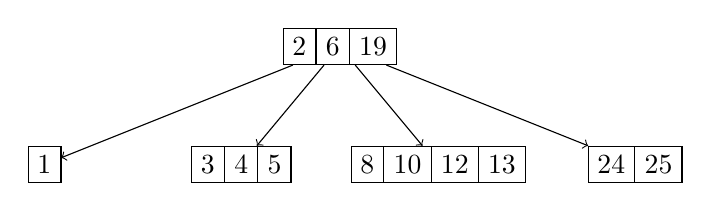
\begin{tikzpicture}
					\tikzstyle{bplus}=[rectangle split, rectangle split horizontal,rectangle split ignore empty parts,draw]
					\tikzstyle{every node}=[bplus]
					\tikzstyle{level 1}=[sibling distance=60mm]
					\tikzstyle{level 2}=[sibling distance=15mm]
					
					\node {2 \nodepart{two} 6 \nodepart{three}19} [->]
					child[sibling distance = 25mm] {node {1}}
					child[sibling distance = 25mm] {node {3 \nodepart{two}4 \nodepart{three} 5}}
					child[sibling distance = 25mm]{ node{ 8 \nodepart{two}10 \nodepart{three}12 \nodepart{four}13}}
					child[sibling distance = 25mm]{ node{24  \nodepart {two} 25}}
					
					;\end{tikzpicture}
			\\Breaking 10 and moving it up.\\
					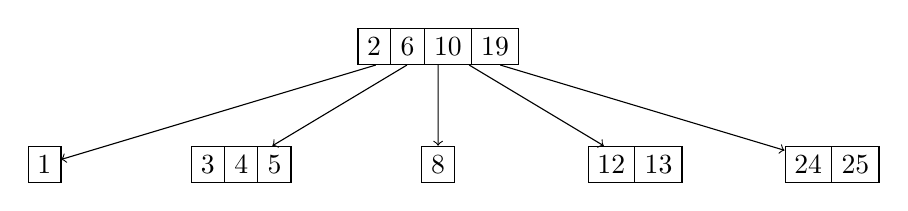
\begin{tikzpicture}
					\tikzstyle{bplus}=[rectangle split, rectangle split horizontal,rectangle split ignore empty parts,draw]
					\tikzstyle{every node}=[bplus]
					\tikzstyle{level 1}=[sibling distance=60mm]
					\tikzstyle{level 2}=[sibling distance=15mm]
					
					\node {2 \nodepart{two} 6 \nodepart{three}10 \nodepart{four}19} [->]
					child[sibling distance = 25mm] {node {1}}
					child[sibling distance = 25mm] {node {3 \nodepart{two}4 \nodepart{three} 5}}
					child[sibling distance = 25mm]{ node{ 8 }}
					child[sibling distance = 25mm]{node {12 \nodepart{two}13}}
					child[sibling distance = 25mm]{ node{24  \nodepart {two} 25}}
					
					;\end{tikzpicture}
			\\Breaking 6 and moving it up.\\
			\begin{center}
					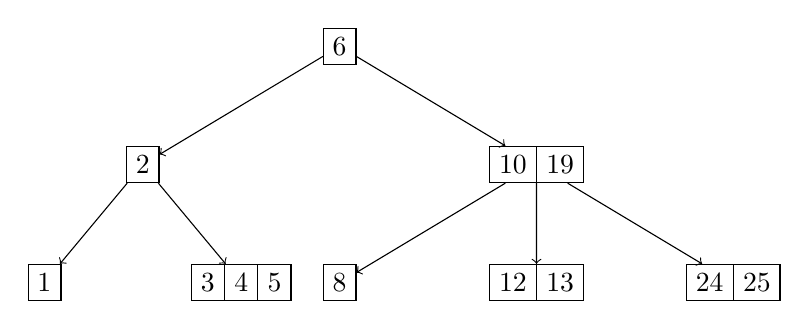
\begin{tikzpicture}
					\tikzstyle{bplus}=[rectangle split, rectangle split horizontal,rectangle split ignore empty parts,draw]
					\tikzstyle{every node}=[bplus]
					\tikzstyle{level 1}=[sibling distance=50mm]
					\tikzstyle{level 2}=[sibling distance=15mm]
					\node {6}[->]
					child{node {2}
						child[sibling distance = 25mm] {node {1}}
						child[sibling distance = 25mm] {node {3 \nodepart{two}4 \nodepart{three} 5}}
					}
					child{ node{ 10 \nodepart{two}19 }
						child[sibling distance = 25mm]{ node{ 8 }}
						child[sibling distance = 25mm]{node {12 \nodepart{two}13}}
						child[sibling distance = 25mm]{ node{24  \nodepart {two} 25}}
					}
					
					;\end{tikzpicture}
				\end{center}
			\item Insert(21) \textit{trivial}
			\begin{center}
				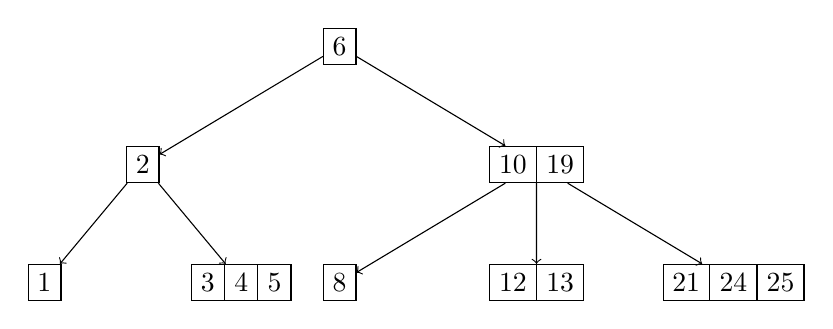
\begin{tikzpicture}
				\tikzstyle{bplus}=[rectangle split, rectangle split horizontal,rectangle split ignore empty parts,draw]
				\tikzstyle{every node}=[bplus]
				\tikzstyle{level 1}=[sibling distance=50mm]
				\tikzstyle{level 2}=[sibling distance=15mm]
				\node {6}[->]
				child{node {2}
					child[sibling distance = 25mm] {node {1}}
					child[sibling distance = 25mm] {node {3 \nodepart{two}4 \nodepart{three} 5}}
				}
				child{ node{ 10 \nodepart{two}19 }
					child[sibling distance = 25mm]{ node{ 8 }}
					child[sibling distance = 25mm]{node {12 \nodepart{two}13}}
					child[sibling distance = 25mm]{ node{21 \nodepart{two}24  \nodepart {three} 25}}
				}
				
				;\end{tikzpicture}
			\end{center}
		\item Insert(23)
			\begin{center}
				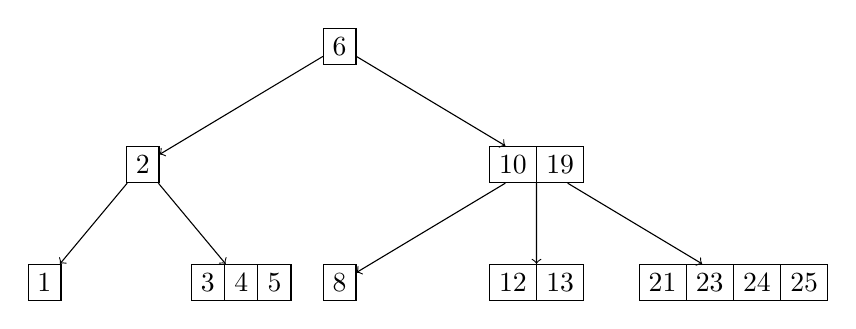
\begin{tikzpicture}
				\tikzstyle{bplus}=[rectangle split, rectangle split horizontal,rectangle split ignore empty parts,draw]
				\tikzstyle{every node}=[bplus]
				\tikzstyle{level 1}=[sibling distance=50mm]
				\tikzstyle{level 2}=[sibling distance=15mm]
				\node {6}[->]
				child{node {2}
					child[sibling distance = 25mm] {node {1}}
					child[sibling distance = 25mm] {node {3 \nodepart{two}4 \nodepart{three} 5}}
				}
				child{ node{ 10 \nodepart{two}19 }
					child[sibling distance = 25mm]{ node{ 8 }}
					child[sibling distance = 25mm]{node {12 \nodepart{two}13}}
					child[sibling distance = 25mm]{ node{21 \nodepart{two}23 \nodepart {three} 24 \nodepart{four}25}}
				}
				
				;\end{tikzpicture}
			\end{center}
		Breaking 23 and moving it up.
			\begin{center}
				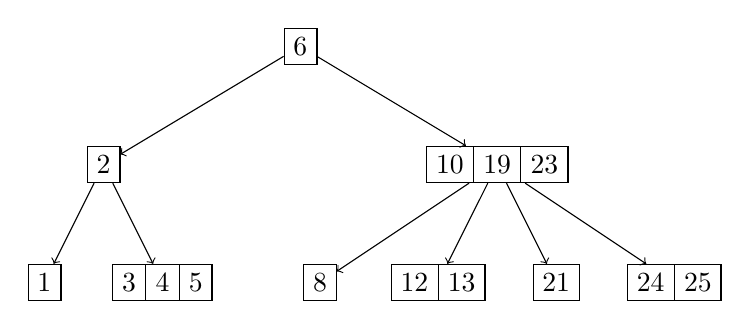
\begin{tikzpicture}
				\tikzstyle{bplus}=[rectangle split, rectangle split horizontal,rectangle split ignore empty parts,draw]
				\tikzstyle{every node}=[bplus]
				\tikzstyle{level 1}=[sibling distance=50mm]
				\tikzstyle{level 2}=[sibling distance=15mm]
				\node {6}[->]
				child{node {2}
					child[sibling distance = 15mm] {node {1}}
					child[sibling distance = 15mm] {node {3 \nodepart{two}4 \nodepart{three} 5}}
				}
				child{ node{ 10 \nodepart{two}19 \nodepart{three}23}
					child[sibling distance = 15mm]{ node{ 8 }}
					child[sibling distance = 15mm]{node {12 \nodepart{two}13}}
					child[sibling distance = 15mm]{node {21}}
					child[sibling distance = 15mm]{ node{24 \nodepart{two}25}}
				}
				
				;\end{tikzpicture}
			\end{center}
		\item Insert(22) \textit{trivial}\\
			\begin{center}
				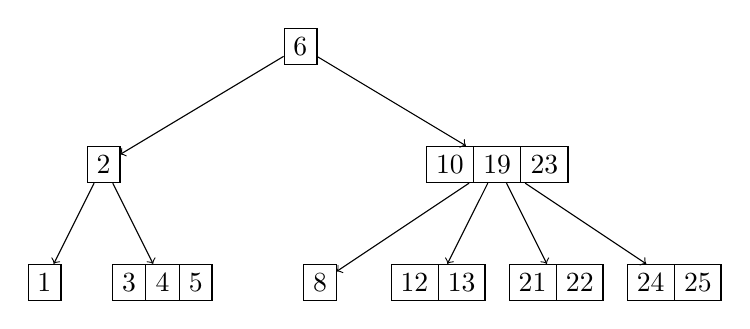
\begin{tikzpicture}
				\tikzstyle{bplus}=[rectangle split, rectangle split horizontal,rectangle split ignore empty parts,draw]
				\tikzstyle{every node}=[bplus]
				\tikzstyle{level 1}=[sibling distance=50mm]
				\tikzstyle{level 2}=[sibling distance=15mm]
				\node {6}[->]
				child{node {2}
					child[sibling distance = 15mm] {node {1}}
					child[sibling distance = 15mm] {node {3 \nodepart{two}4 \nodepart{three} 5}}
				}
				child{ node{ 10 \nodepart{two}19 \nodepart{three}23}
					child[sibling distance = 15mm]{ node{ 8 }}
					child[sibling distance = 15mm]{node {12 \nodepart{two}13}}
					child[sibling distance = 15mm]{node {21 \nodepart{two}22}}
					child[sibling distance = 15mm]{ node{24 \nodepart{two}25}}
				}
				
				;\end{tikzpicture}
			\end{center}
	\end{enumerate}
	\item Red-Black Tree
	\begin{enumerate}
		\item Insert (1)\\
		Node is added as red but if node is root, change color to black and done.\\
			\begin{center}
			
\begin{tikzpicture}[->,>=stealth',level/.style={sibling distance = 25mm/#1,
				level distance = 1cm}] 
			\node [arn_n] {1}
			
			;\end{tikzpicture}
			\end{center}
			
		\item Insert(24)\\
		24 is added as red, and its parent is black therefore done.
			\begin{center}
				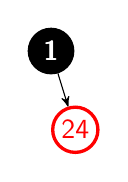
\begin{tikzpicture}[->,>=stealth',level/.style={sibling distance = 25mm/#1,
					level distance = 1cm}] 
				\node [arn_n] {1}
				child{node[arn_r][right]{24}}
				;\end{tikzpicture}
			\end{center}
		\item Insert(2)\\
		2 is added as red, and there is a conflict.
			\begin{center}
				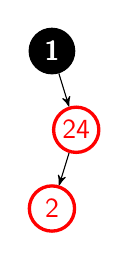
\begin{tikzpicture}[->,>=stealth',level/.style={sibling distance = 25mm/#1,
					level distance = 1cm}] 
				\node [arn_n] {1}
				child{node[arn_r][right]{24}
					child{node[arn_r][left]{2}}
					}
				;\end{tikzpicture}
			\end{center}
		Since no uncle, we assume uncle is black. Case is right-left, therefore we  RotateRight(24)
			\begin{center}
				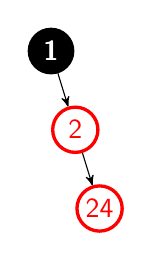
\begin{tikzpicture}[->,>=stealth',level/.style={sibling distance = 25mm/#1,
					level distance = 1cm}] 
				\node [arn_n] {1}
				child{node[arn_r][right]{2}
					child{node[arn_r][right]{24}}
				}	
				;\end{tikzpicture}
			\end{center}
		Fix (24) and case is right right. Therefore color 2 black, 1 red and left-rotate(1)
			\begin{center}
				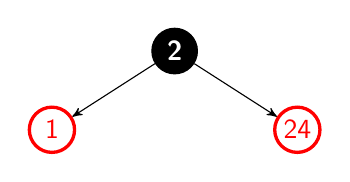
\begin{tikzpicture}[->,>=stealth',level/.style={sibling distance = 25mm/#1,
					level distance = 1cm}] 
				\node [arn_n] {2}
				child{node[arn_r][left]{1}}
				child{node[arn_r][right]{24}}
				
				;\end{tikzpicture}
			\end{center}
	\item Insert(6)\\
		6 is inserted to the left of 24, with red as default. We get a conflict.
		\begin{center}
			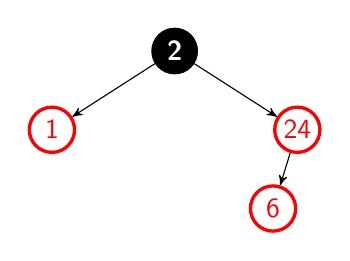
\begin{tikzpicture}[->,>=stealth',level/.style={sibling distance = 25mm/#1,
				level distance = 1cm}] 
			\node [arn_n] {2}
			child{node[arn_r][left]{1}}
			child{node[arn_r][right]{24}
				child{node[arn_r][left]{6}}
			}
			
			;\end{tikzpicture}
		\end{center}
		Since uncle is red, we just color parent and uncle black, and grandparent red. Since grandparent is root, fix(grandparent) would make grandparent black.
		\begin{center}
			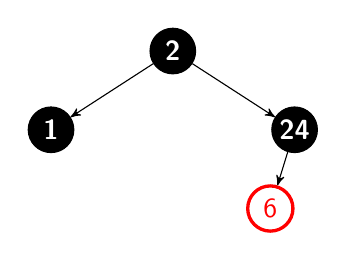
\begin{tikzpicture}[->,>=stealth',level/.style={sibling distance = 25mm/#1,
				level distance = 1cm}] 
			\node [arn_n] {2}
			child{node[arn_n][left]{1}}
			child{node[arn_n][right]{24}
				child{node[arn_r][left]{6}}
			}
			
			;\end{tikzpicture}
		\end{center}
	\item Insert(4)\\
	Since inserted 4 is red, we get a conflict.
	\begin{center}
		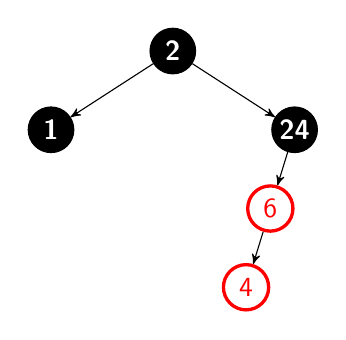
\begin{tikzpicture}[->,>=stealth',level/.style={sibling distance = 25mm/#1,
			level distance = 1cm}] 
		\node [arn_n] {2}
		child{node[arn_n][left]{1}}
		child{node[arn_n][right]{24}
			child{node[arn_r][left]{6}
				child{node[arn_r][left]{4}}
			}
		}
		
		;\end{tikzpicture}
	\end{center}
	Since uncle is black and the inserted case is left left, we change parent to black, grandparent to red, and rotateRight(g)
		\begin{center}
			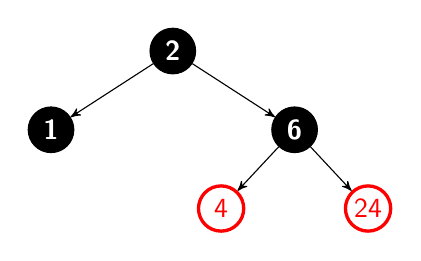
\begin{tikzpicture}[->,>=stealth',level/.style={sibling distance = 25mm/#1,
				level distance = 1cm}] 
			\node [arn_n] {2}
			child{node[arn_n][left]{1}}
			child{node[arn_n][right]{6}
				child{node[arn_r][left]{4}}
				child{node[arn_r][right]{24}}
			}
			;\end{tikzpicture}
		\end{center}
	\item Insert(12)
	Inserted 12 is red and to the left of 24.
		\begin{center}
			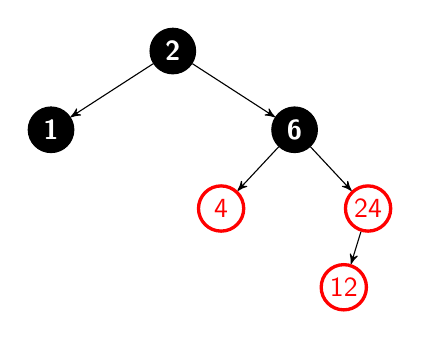
\begin{tikzpicture}[->,>=stealth',level/.style={sibling distance = 25mm/#1,
				level distance = 1cm}] 
			\node [arn_n] {2}
			child{node[arn_n][left]{1}}
			child{node[arn_n][right]{6}
				child{node[arn_r][left]{4}}
				child{node[arn_r][right]{24}
					child{node[arn_r][left]{12}}
				}
			}
			;\end{tikzpicture}
		\end{center}
	Inserted case is left-right and uncle is red. Therefore we color p and u black, g red, and fix(g). g has a black parent, therefore we stop there.	
		
		\begin{center}
			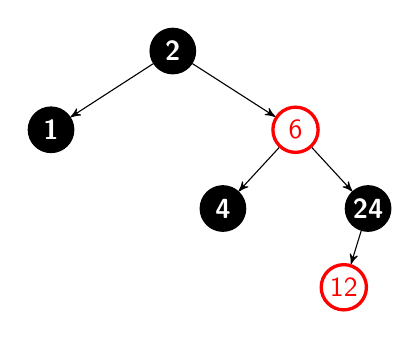
\begin{tikzpicture}[->,>=stealth',level/.style={sibling distance = 25mm/#1,
				level distance = 1cm}] 
			\node [arn_n] {2}
			child{node[arn_n][left]{1}}
			child{node[arn_r][right]{6}
				child{node[arn_n][left]{4}}
				child{node[arn_n][right]{24}
					child{node[arn_r][left]{12}}
				}
			}
			;\end{tikzpicture}
		\end{center}
	\item Insert(25)\\
	25 is red and is inserted to the right of 24. Trivial.
		\begin{center}
			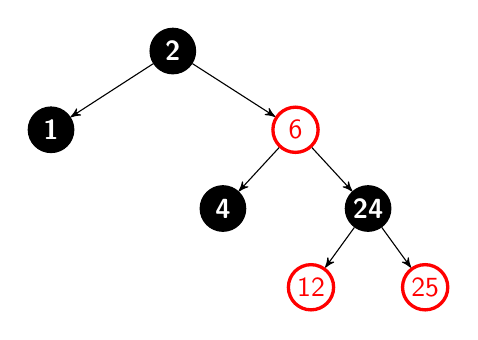
\begin{tikzpicture}[->,>=stealth',level/.style={sibling distance = 25mm/#1,
				level distance = 1cm}] 
			\node [arn_n] {2}
			child{node[arn_n][left]{1}}
			child{node[arn_r][right]{6}
				child{node[arn_n][left]{4}}
				child{node[arn_n][right]{24}
					child{node[arn_r][left]{12}}
					child{node[arn_r][right]{25}}
				}
			}
			;\end{tikzpicture}
		\end{center}
	\item Insert(19)\\
		Inserted to the right of 12 which results in a conflic.
		\begin{center}
			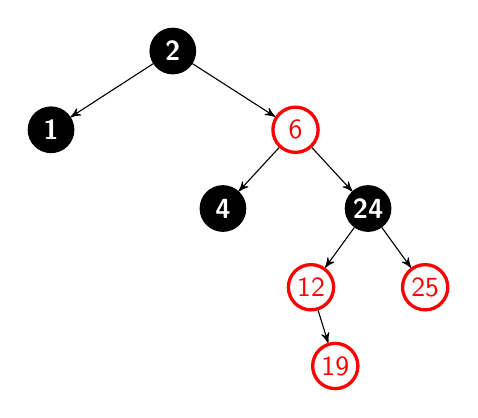
\begin{tikzpicture}[->,>=stealth',level/.style={sibling distance = 25mm/#1,
				level distance = 1cm}] 
			\node [arn_n] {2}
			child{node[arn_n][left]{1}}
			child{node[arn_r][right]{6}
				child{node[arn_n][left]{4}}
				child{node[arn_n][right]{24}
					child{node[arn_r][left]{12}
					child{node[arn_r][right]{19}}
					}
					child{node[arn_r][right]{25}}
				}
			}
			;\end{tikzpicture}
		\end{center}
		Since the uncle is red, we color p and u black, g red and fix(g).
		\begin{center}
			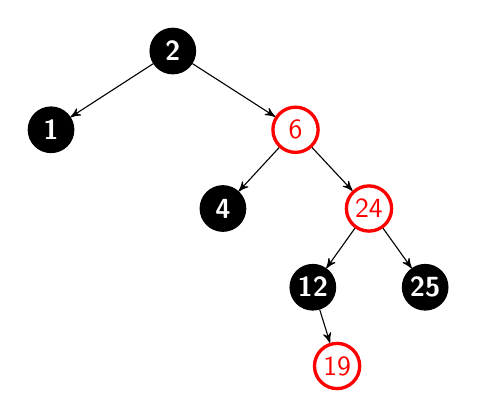
\begin{tikzpicture}[->,>=stealth',level/.style={sibling distance = 25mm/#1,
				level distance = 1cm}] 
			\node [arn_n] {2}
			child{node[arn_n][left]{1}}
			child{node[arn_r][right]{6}
				child{node[arn_n][left]{4}}
				child{node[arn_r][right]{24}
					child{node[arn_n][left]{12}
						child{node[arn_r][right]{19}}
					}
					child{node[arn_n][right]{25}}
				}
			}
			;\end{tikzpicture}
		\end{center}
	24 has black uncle and is right right case. Therefore we color p (6) black, g (2) red and rotateLeft(2)
	\begin{center}
		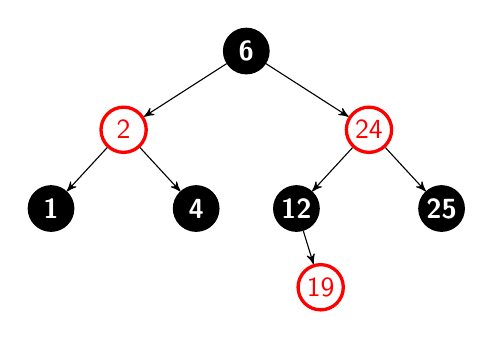
\begin{tikzpicture}[->,>=stealth',level/.style={sibling distance = 25mm/#1,
			level distance = 1cm}] 
		\node [arn_n] {6}
		child{node[arn_r][left]{2}
			child{node[arn_n][left]{1}}
			child{node[arn_n][right]{4}}
		}
		child{node[arn_r][right]{24}
			child{node[arn_n][left]{12}
				child{node[arn_r][right]{19}}
			}
			child{node[arn_n][right]{25}}
			}
		;\end{tikzpicture}
	\end{center}
	\item Insert(10)\\
	10 is inserted to the left of 12. Since the parent is black, we are done. This case is trivial.
	\begin{center}
		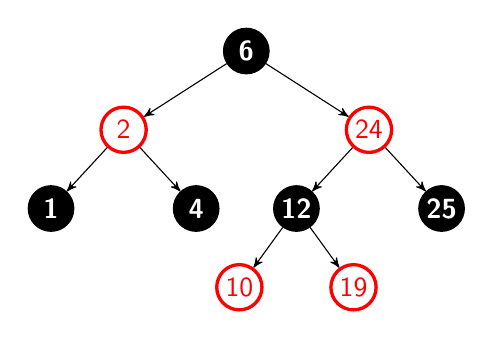
\begin{tikzpicture}[->,>=stealth',level/.style={sibling distance = 25mm/#1,
			level distance = 1cm}] 
		\node [arn_n] {6}
		child{node[arn_r][left]{2}
			child{node[arn_n][left]{1}}
			child{node[arn_n][right]{4}}
		}
		child{node[arn_r][right]{24}
			child{node[arn_n][left]{12}
				child{node[arn_r][left]{10}}
				child{node[arn_r][right]{19}}
			}
			child{node[arn_n][right]{25}}
		}
		;\end{tikzpicture}
	\end{center}
	\item Insert(5)\\
	5 is inserted to the right of 4. Since the parent is black, we are done. This case is trivial.
	\begin{center}
		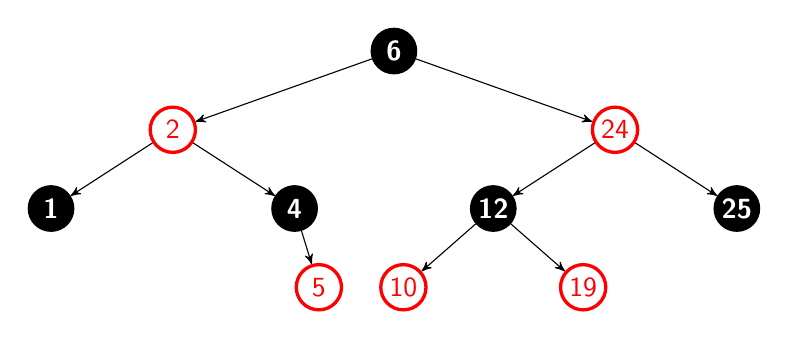
\begin{tikzpicture}[->,>=stealth',level/.style={sibling distance = 5cm/#1,
			level distance = 1cm}] 
		\node [arn_n] {6}
		child{node[arn_r][left]{2}
			child{node[arn_n][left]{1}}
			child{node[arn_n][right]{4}
				child{node[arn_r][right]{5}}	
				}
		}
		child{node[arn_r][right]{24}
			child{node[arn_n][left]{12}
				child{node[arn_r][left]{10}}
				child{node[arn_r][right]{19}}
			}
			child{node[arn_n][right]{25}}
		}
		;\end{tikzpicture}
	\end{center}
	\item Insert(3)\\
	3 is inserted to the left of 4. Since the parent is black, we are done. This case is trivial.
		
	\begin{center}
		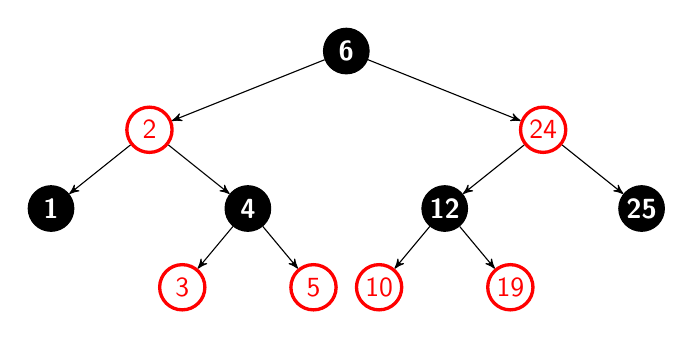
\begin{tikzpicture}[->,>=stealth',level/.style={sibling distance = 5cm/#1,
			level distance = 1cm}] 
		\node [arn_n] {6}
		child{node[arn_r]{2}
			child{node[arn_n]{1}}
			child{node[arn_n]{4}
				child{node[arn_r]{3}}
				child{node[arn_r]{5}}	
			}
		}
		child{node[arn_r]{24}
			child{node[arn_n]{12}
				child{node[arn_r]{10}}
				child{node[arn_r]{19}}
			}
			child{node[arn_n]{25}}
		}
		;\end{tikzpicture}
	\end{center}
	\item Insert(13)\\
	13 would be inserted to the left of 19. There will be a conflict.
		\begin{center}
			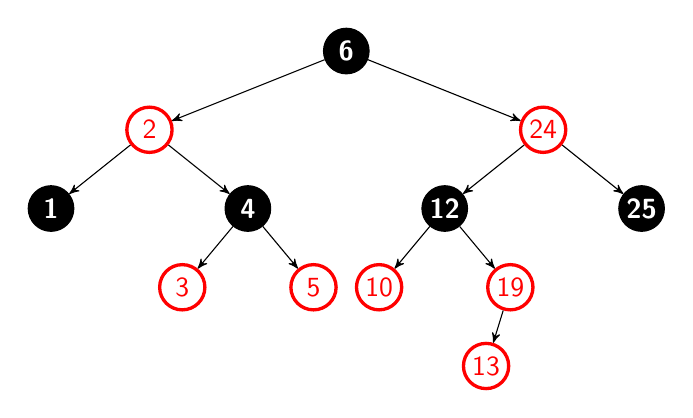
\begin{tikzpicture}[->,>=stealth',level/.style={sibling distance = 5cm/#1,
				level distance = 1cm}] 
			\node [arn_n] {6}
			child{node[arn_r]{2}
				child{node[arn_n]{1}}
				child{node[arn_n]{4}
					child{node[arn_r]{3}}
					child{node[arn_r]{5}}	
				}
			}
			child{node[arn_r]{24}
				child{node[arn_n]{12}
					child{node[arn_r]{10}}
					child{node[arn_r]{19}
						child{node[arn_r][left]{13}}
					}	
					}
				child{node[arn_n]{25}}
			}
			;\end{tikzpicture}
		\end{center}
	13's uncle is red, therefore, we color 19 and 10 black, and 12 red and call fix(12)
	\begin{center}
		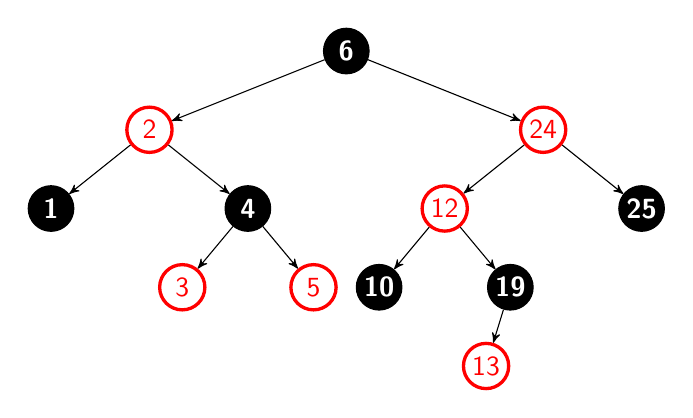
\begin{tikzpicture}[->,>=stealth',level/.style={sibling distance = 5cm/#1,
			level distance = 1cm}] 
		\node [arn_n] {6}
		child{node[arn_r]{2}
			child{node[arn_n]{1}}
			child{node[arn_n]{4}
				child{node[arn_r]{3}}
				child{node[arn_r]{5}}	
			}
		}
		child{node[arn_r]{24}
			child{node[arn_r]{12}
				child{node[arn_n]{10}}
				child{node[arn_n]{19}
					child{node[arn_r][left]{13}}
				}	
			}
			child{node[arn_n]{25}}
		}
		;\end{tikzpicture}
	\end{center}
	12's uncle is red and therefore, we color 24 and 2 black, and 6 red, and call fix(6). Since 6 is root, it is changed to black and we are done. (We have not shown one step here.)
	\begin{center}
		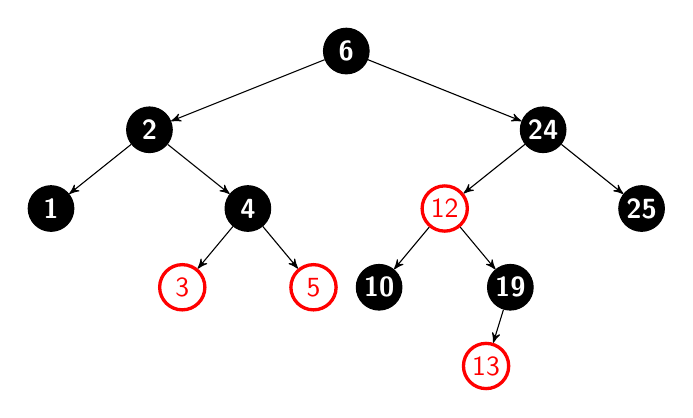
\begin{tikzpicture}[->,>=stealth',level/.style={sibling distance = 5cm/#1,
			level distance = 1cm}] 
		\node [arn_n] {6}
		child{node[arn_n]{2}
			child{node[arn_n]{1}}
			child{node[arn_n]{4}
				child{node[arn_r]{3}}
				child{node[arn_r]{5}}	
			}
		}
		child{node[arn_n]{24}
			child{node[arn_r]{12}
				child{node[arn_n]{10}}
				child{node[arn_n]{19}
					child{node[arn_r][left]{13}}
				}	
			}
			child{node[arn_n]{25}}
		}
		;\end{tikzpicture}
	\end{center}
	\item Insert(8)\\
	8 will go to the left of 10. Since the parent is black, this case is trivial.
	\begin{center}
		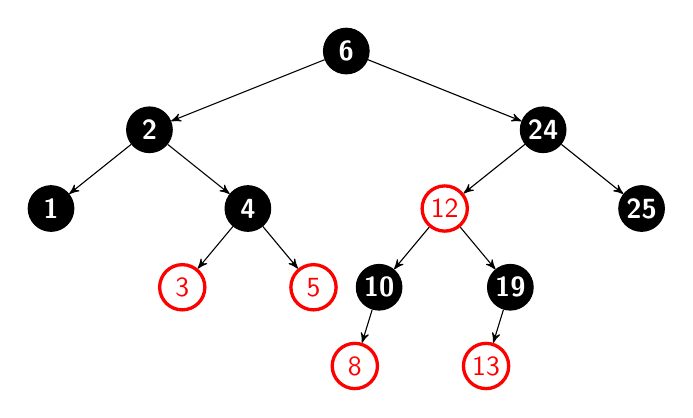
\begin{tikzpicture}[->,>=stealth',level/.style={sibling distance = 5cm/#1,
			level distance = 1cm}] 
		\node [arn_n] {6}
		child{node[arn_n]{2}
			child{node[arn_n]{1}}
			child{node[arn_n]{4}
				child{node[arn_r]{3}}
				child{node[arn_r]{5}}	
			}
		}
		child{node[arn_n]{24}
			child{node[arn_r]{12}
				child{node[arn_n]{10}
					child{node[arn_r][left]{8}}
				}
				child{node[arn_n]{19}
					child{node[arn_r][left]{13}}
				}	
			}
			child{node[arn_n]{25}}
		}
		;\end{tikzpicture}
	\end{center}
	\item Insert(21)\\
	21 will be inserted to the right of 19. Since its parent is black, this case is trivial.
	\begin{center}
		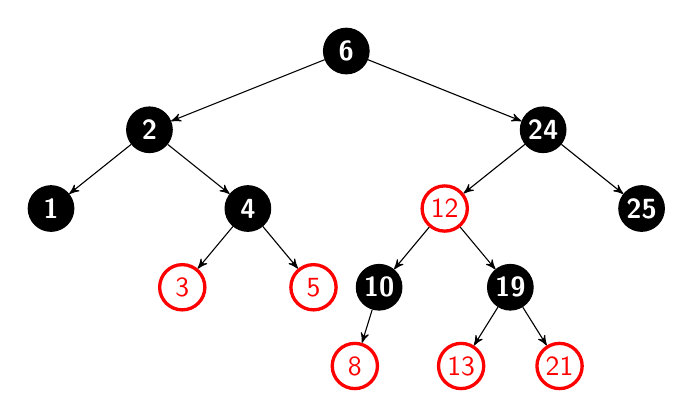
\begin{tikzpicture}[->,>=stealth',level/.style={sibling distance = 5cm/#1,
			level distance = 1cm}] 
		\node [arn_n] {6}
		child{node[arn_n]{2}
			child{node[arn_n]{1}}
			child{node[arn_n]{4}
				child{node[arn_r]{3}}
				child{node[arn_r]{5}}	
			}
		}
		child{node[arn_n]{24}
			child{node[arn_r]{12}
				child{node[arn_n]{10}
					child{node[arn_r][left]{8}}
				}
				child{node[arn_n]{19}
					child{node[arn_r]{13}}
					child{node[arn_r]{21}}
				}	
			}
			child{node[arn_n]{25}}
		}
		;\end{tikzpicture}
	\end{center}
	\item Insert(23)\\
	23 will be inserted to the right of 21. There will be a conflict.
	\begin{center}
		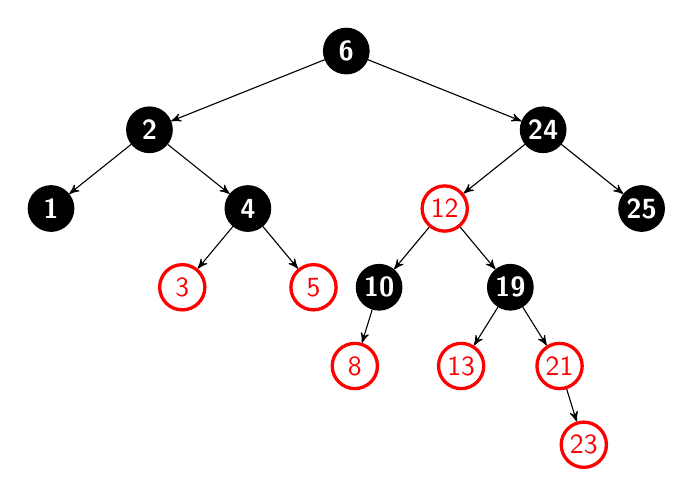
\begin{tikzpicture}[->,>=stealth',level/.style={sibling distance = 5cm/#1,
			level distance = 1cm}] 
		\node [arn_n] {6}
		child{node[arn_n]{2}
			child{node[arn_n]{1}}
			child{node[arn_n]{4}
				child{node[arn_r]{3}}
				child{node[arn_r]{5}}	
			}
		}
		child{node[arn_n]{24}
			child{node[arn_r]{12}
				child{node[arn_n]{10}
					child{node[arn_r][left]{8}}
				}
				child{node[arn_n]{19}
					child{node[arn_r]{13}}
					child{node[arn_r]{21}
						child{node[arn_r][right]{23}}
						}
				}	
			}
			child{node[arn_n]{25}}
		}
		
		;\end{tikzpicture}
	\end{center}
	23 has red uncle, therefore we change 21 to black, 13 to black, 19 to red and fix(12).
	\begin{center}
		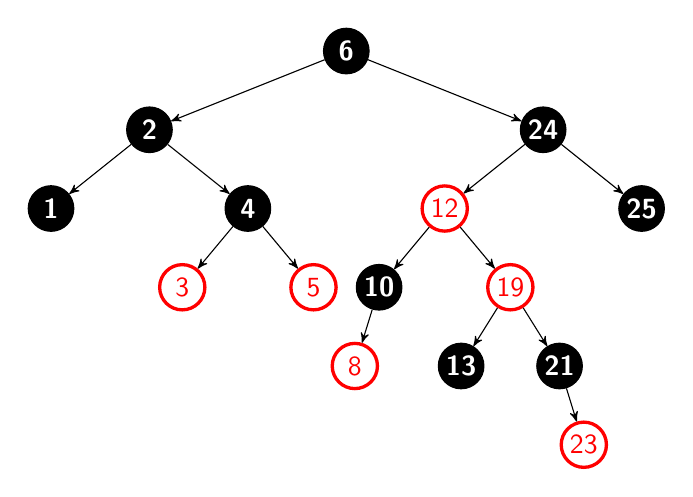
\begin{tikzpicture}[->,>=stealth',level/.style={sibling distance = 5cm/#1,
			level distance = 1cm}] 
		\node [arn_n] {6}
		child{node[arn_n]{2}
			child{node[arn_n]{1}}
			child{node[arn_n]{4}
				child{node[arn_r]{3}}
				child{node[arn_r]{5}}	
			}
		}
		child{node[arn_n]{24}
			child{node[arn_r]{12}
				child{node[arn_n]{10}
					child{node[arn_r][left]{8}}
				}
				child{node[arn_r]{19}
					child{node[arn_n]{13}}
					child{node[arn_n]{21}
						child{node[arn_r][right]{23}}
					}
				}	
			}
			child{node[arn_n]{25}}
		}
		
		;\end{tikzpicture}
	\end{center}
	19 has black uncle, and its case is left-right. Therefore we rotateLeft(12) (12 is its parent)
		\begin{center}
			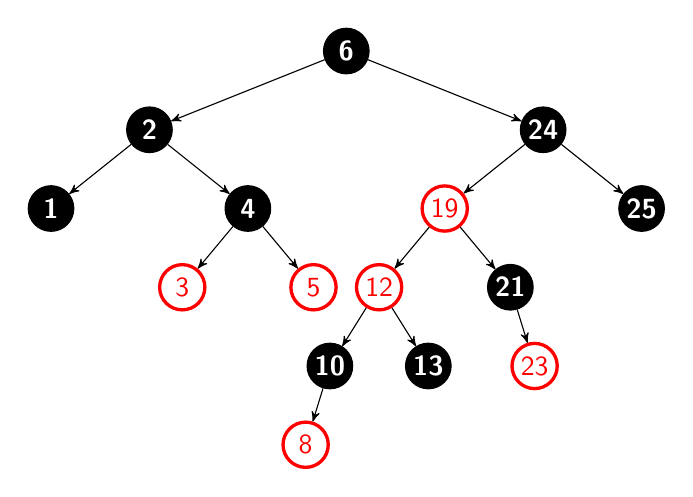
\begin{tikzpicture}[->,>=stealth',level/.style={sibling distance = 5cm/#1,
				level distance = 1cm}] 
			\node [arn_n] {6}
			child{node[arn_n]{2}
				child{node[arn_n]{1}}
				child{node[arn_n]{4}
					child{node[arn_r]{3}}
					child{node[arn_r]{5}}	
				}
			}
			child{node[arn_n]{24}
				child{node[arn_r]{19}
					child{node[arn_r]{12}
						child{node[arn_n]{10}
							child{node[arn_r][left]{8}}
						}
						child{node[arn_n]{13}}
					}	
					child{node[arn_n]{21}
						child{node[arn_r][right]{23}}
					}
				}	
				child{node[arn_n]{25}}
			}
			
			;\end{tikzpicture}
		\end{center}
	12 has black uncle and is left left case. Therefore we color 19 black, 24 red and rotateRight(24)
		\begin{center}
			\begin{tikzpicture}[->,>=stealth',level/.style={sibling distance = 5cm/#1,
				level distance = 1cm}] 
			\node [arn_n] {6}
			child{node[arn_n]{2}
				child{node[arn_n]{1}}
				child{node[arn_n]{4}
					child{node[arn_r]{3}}
					child{node[arn_r]{5}}	
				}
			}
			child{node[arn_n]{19}
				child{node[arn_r]{12}
						child{node[arn_n]{10}
							child{node[arn_r][left]{8}}
						}
						child{node[arn_n]{13}}
					}	
					child{node[arn_r]{24}
						child{node[arn_n]{21}
							child{node[arn_r][right]{23}}
						}	
						child{node[arn_n]{25}}
					}
				}
			
			;\end{tikzpicture}
		\end{center}
	\item Insert(22)\\
	22 would be inserted to the left of 23. There will be a conflict.
	\begin{center}
		\begin{tikzpicture}[->,>=stealth',level/.style={sibling distance = 5cm/#1,
			level distance = 1cm}] 
		\node [arn_n] {6}
		child{node[arn_n]{2}
			child{node[arn_n]{1}}
			child{node[arn_n]{4}
				child{node[arn_r]{3}}
				child{node[arn_r]{5}}	
			}
		}
		child{node[arn_n]{19}
			child{node[arn_r]{12}
				child{node[arn_n]{10}
					child{node[arn_r][left]{8}}
				}
				child{node[arn_n]{13}}
			}	
			child{node[arn_r]{24}
				child{node[arn_n]{21}
					child{node[arn_r][right]{23}
						child{node[arn_r][left]{22}}
					}
				}	
				child{node[arn_n]{25}}
			}
		}
		
		;\end{tikzpicture}
	\end{center}
	Since uncle is (non-existent) black, we see that case is right-left. We rotateRight(23) (23 is parent) and fix(23).
	\begin{center}
		\begin{tikzpicture}[->,>=stealth',level/.style={sibling distance = 5cm/#1,
			level distance = 1cm}] 
		\node [arn_n] {6}
		child{node[arn_n]{2}
			child{node[arn_n]{1}}
			child{node[arn_n]{4}
				child{node[arn_r]{3}}
				child{node[arn_r]{5}}	
			}
		}
		child{node[arn_n]{19}
			child{node[arn_r]{12}
				child{node[arn_n]{10}
					child{node[arn_r][left]{8}}
				}
				child{node[arn_n]{13}}
			}	
			child{node[arn_r]{24}
				child{node[arn_n]{21}
					child{node[arn_r][right]{22}
						child{node[arn_r][right]{23}}
					}
				}	
				child{node[arn_n]{25}}
			}
		}
		
		;\end{tikzpicture}
	\end{center}
	23 case is right right, and therefore, we change color of 22 to black, 21 to red, and rotateLeft(21) (21 is grandparent)
	\begin{center}
		\begin{tikzpicture}[->,>=stealth',level/.style={sibling distance = 5cm/#1,
			level distance = 1cm}] 
		\node [arn_n] {6}
		child{node[arn_n]{2}
			child{node[arn_n]{1}}
			child{node[arn_n]{4}
				child{node[arn_r]{3}}
				child{node[arn_r]{5}}	
			}
		}
		child{node[arn_n]{19}
			child{node[arn_r]{12}
				child{node[arn_n]{10}
					child{node[arn_r][left]{8}}
				}
				child{node[arn_n]{13}}
			}	
			child{node[arn_r]{24}
				child{node[arn_n]{22}
					child{node[arn_r]{21}}
					child{node[arn_r]{23}}
				}	
				child{node[arn_n]{25}}
			}
		}
		
		;\end{tikzpicture}
	\end{center}
	At this point we see that all 4 properties of the rb tree are balanced. Each node has black height 4, root node is black, red has black children, and each node is either red or black.
	\end{enumerate}	
\end{enumerate}
		
\section*{Problem 3. Deletion}
\begin{enumerate}
	\item Original Tree (for reference purposes)
		\begin{center}
			\begin{tikzpicture}
			\tikzstyle{bplus}=[rectangle split, rectangle split horizontal,rectangle split ignore empty parts,draw]
			\tikzstyle{every node}=[bplus]
			\tikzstyle{level 1}=[sibling distance=50mm]
			\tikzstyle{level 2}=[sibling distance=15mm]
			\node {6}[->]
			child{node {2}
				child[sibling distance = 15mm] {node {1}}
				child[sibling distance = 15mm] {node {3 \nodepart{two}4 \nodepart{three} 5}}
			}
			child{ node{ 10 \nodepart{two}19 \nodepart{three}23}
				child[sibling distance = 15mm]{ node{ 8 }}
				child[sibling distance = 15mm]{node {12 \nodepart{two}13}}
				child[sibling distance = 15mm]{node {21 \nodepart{two}22}}
				child[sibling distance = 15mm]{ node{24 \nodepart{two}25}}
			}
			
			;\end{tikzpicture}
		\end{center}
	\item Remove(13) \textit{trivial}
	\begin{center}
		\begin{tikzpicture}
		\tikzstyle{bplus}=[rectangle split, rectangle split horizontal,rectangle split ignore empty parts,draw]
		\tikzstyle{every node}=[bplus]
		\tikzstyle{level 1}=[sibling distance=50mm]
		\tikzstyle{level 2}=[sibling distance=15mm]
		\node {6}[->]
		child{node {2}
			child[sibling distance = 15mm] {node {1}}
			child[sibling distance = 15mm] {node {3 \nodepart{two}4 \nodepart{three} 5}}
		}
		child{ node{ 10 \nodepart{two}19 \nodepart{three}23}
			child[sibling distance = 15mm]{ node{ 8 }}
			child[sibling distance = 15mm]{node {12}}
			child[sibling distance = 15mm]{node {21 \nodepart{two}22}}
			child[sibling distance = 15mm]{ node{24 \nodepart{two}25}}
		}
		
		;\end{tikzpicture}
	\end{center}
	\item Remove(12)
	\begin{center}
		\begin{tikzpicture}
		\tikzstyle{bplus}=[rectangle split, rectangle split horizontal,rectangle split ignore empty parts,draw]
		\tikzstyle{every node}=[bplus]
		\tikzstyle{level 1}=[sibling distance=50mm]
		\tikzstyle{level 2}=[sibling distance=15mm]
		\node {6}[->]
		child{node {2}
			child[sibling distance = 15mm] {node {1}}
			child[sibling distance = 15mm] {node {3 \nodepart{two}4 \nodepart{three} 5}}
		}
		child{ node{ 10 \nodepart{two}19 \nodepart{three}23}
			child[sibling distance = 15mm]{ node{ 8 }}
			child[sibling distance = 15mm]{}
			child[sibling distance = 15mm]{node {21 \nodepart{two}22}}
			child[sibling distance = 15mm]{ node{24 \nodepart{two}25}}
		}
		
		;\end{tikzpicture}
	\end{center}
	Pushing 19 down and 21 up,
	\begin{center}
		\begin{tikzpicture}
		\tikzstyle{bplus}=[rectangle split, rectangle split horizontal,rectangle split ignore empty parts,draw]
		\tikzstyle{every node}=[bplus]
		\tikzstyle{level 1}=[sibling distance=50mm]
		\tikzstyle{level 2}=[sibling distance=15mm]
		\node {6}[->]
		child{node {2}
			child[sibling distance = 15mm] {node {1}}
			child[sibling distance = 15mm] {node {3 \nodepart{two}4 \nodepart{three} 5}}
		}
		child{ node{ 10 \nodepart{two}21 \nodepart{three}23}
			child[sibling distance = 15mm]{ node{ 8 }}
			child[sibling distance = 15mm]{node{19}}
			child[sibling distance = 15mm]{node {22}}
			child[sibling distance = 15mm]{ node{24 \nodepart{two}25}}
		}
		
		;\end{tikzpicture}
	\end{center}
	
\item Remove(5) \textit{trivial}
	\begin{center}
		\begin{tikzpicture}
		\tikzstyle{bplus}=[rectangle split, rectangle split horizontal,rectangle split ignore empty parts,draw]
		\tikzstyle{every node}=[bplus]
		\tikzstyle{level 1}=[sibling distance=50mm]
		\tikzstyle{level 2}=[sibling distance=15mm]
		\node {6}[->]
		child{node {2}
			child[sibling distance = 15mm] {node {1}}
			child[sibling distance = 15mm] {node {3 \nodepart{two}4}}
		}
		child{ node{ 10 \nodepart{two}21 \nodepart{three}23}
			child[sibling distance = 15mm]{ node{ 8 }}
			child[sibling distance = 15mm]{node{19}}
			child[sibling distance = 15mm]{node {22}}
			child[sibling distance = 15mm]{ node{24 \nodepart{two}25}}
		}
		
		;\end{tikzpicture}
	\end{center}
	
\item Remove(24) \textit{trivial}
	\begin{center}
		\begin{tikzpicture}
		\tikzstyle{bplus}=[rectangle split, rectangle split horizontal,rectangle split ignore empty parts,draw]
		\tikzstyle{every node}=[bplus]
		\tikzstyle{level 1}=[sibling distance=50mm]
		\tikzstyle{level 2}=[sibling distance=15mm]
		\node {6}[->]
		child{node {2}
			child[sibling distance = 15mm] {node {1}}
			child[sibling distance = 15mm] {node {3 \nodepart{two}4}}
		}
		child{ node{ 10 \nodepart{two}21 \nodepart{three}23}
			child[sibling distance = 15mm]{ node{ 8 }}
			child[sibling distance = 15mm]{node{19}}
			child[sibling distance = 15mm]{node {22}}
			child[sibling distance = 15mm]{ node{25}}
		}
		
		;\end{tikzpicture}
	\end{center}
	
\item Remove(8)	
	\begin{center}
	\begin{tikzpicture}
	\tikzstyle{bplus}=[rectangle split, rectangle split horizontal,rectangle split ignore empty parts,draw]
	\tikzstyle{every node}=[bplus]
	\tikzstyle{level 1}=[sibling distance=50mm]
	\tikzstyle{level 2}=[sibling distance=15mm]
	\node {6}[->]
	child{node {2}
		child[sibling distance = 15mm] {node {1}}
		child[sibling distance = 15mm] {node {3 \nodepart{two}4}}
	}
	child{ node{ 10 \nodepart{two}21 \nodepart{three}23}
		child[sibling distance = 15mm]{}
		child[sibling distance = 15mm]{node{19}}
		child[sibling distance = 15mm]{node {22}}
		child[sibling distance = 15mm]{ node{25}}
	}
	
	;\end{tikzpicture}
	\end{center}
Pushing 10 down and bringing 19 up,
	\begin{center}
		\begin{tikzpicture}
		\tikzstyle{bplus}=[rectangle split, rectangle split horizontal,rectangle split ignore empty parts,draw]
		\tikzstyle{every node}=[bplus]
		\tikzstyle{level 1}=[sibling distance=50mm]
		\tikzstyle{level 2}=[sibling distance=15mm]
		\node {6}[->]
		child{node {2}
			child[sibling distance = 15mm] {node {1}}
			child[sibling distance = 15mm] {node {3 \nodepart{two}4}}
		}
		child{ node{ 19 \nodepart{two}21 \nodepart{three}23}
			child[sibling distance = 15mm]{node{10}}
			child[sibling distance = 15mm]{}
			child[sibling distance = 15mm]{node {22}}
			child[sibling distance = 15mm]{ node{25}}
		}
		
		;\end{tikzpicture}
	\end{center}
Pulling 19 down will give us our final tree while 2-3 property is not violated.
\begin{center}
	\begin{tikzpicture}
	\tikzstyle{bplus}=[rectangle split, rectangle split horizontal,rectangle split ignore empty parts,draw]
	\tikzstyle{every node}=[bplus]
	\tikzstyle{level 1}=[sibling distance=50mm]
	\tikzstyle{level 2}=[sibling distance=15mm]
	\node {6}[->]
	child{node {2}
		child[sibling distance = 15mm] {node {1}}
		child[sibling distance = 15mm] {node {3 \nodepart{two}4}}
	}
	child{ node{21 \nodepart{two}23}
		child[sibling distance = 15mm]{node{10 \nodepart{two}19}}
		child[sibling distance = 15mm]{node {22}}
		child[sibling distance = 15mm]{ node{25}}
	}
	
	;\end{tikzpicture}
\end{center}

\end{enumerate}

\end{document}
